%\begin{figure*}[ht!]
%\centering
%\textbf{a) \textit{DaCapo}}\\
%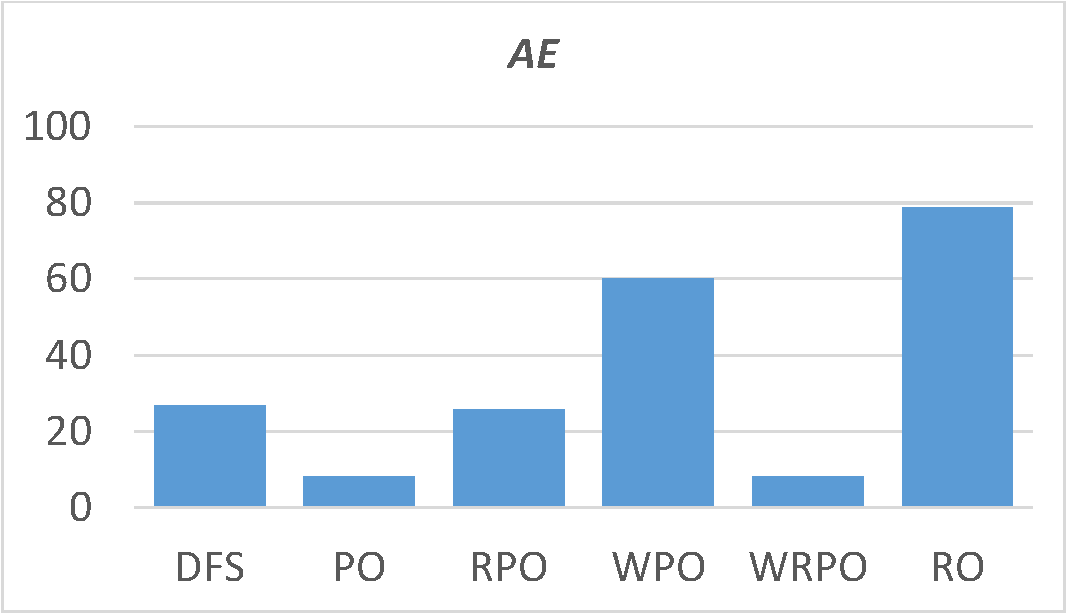
\includegraphics[width=0.32\linewidth]{ecoop-figures/ae-crop.pdf}
%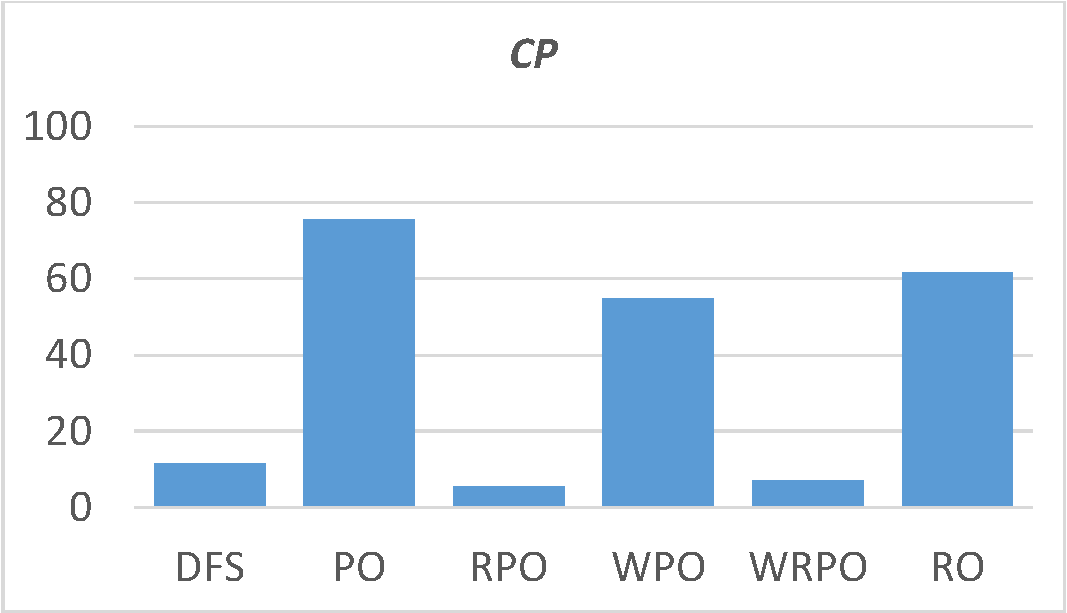
\includegraphics[width=0.32\linewidth]{ecoop-figures/cp-crop.pdf}
%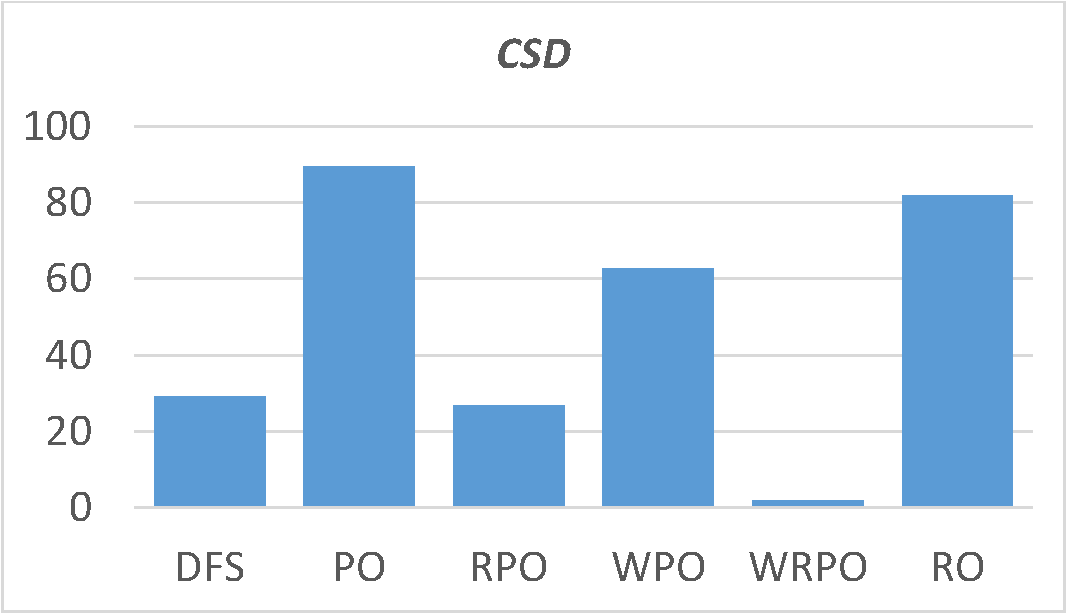
\includegraphics[width=0.32\linewidth]{ecoop-figures/csd-crop.pdf}
%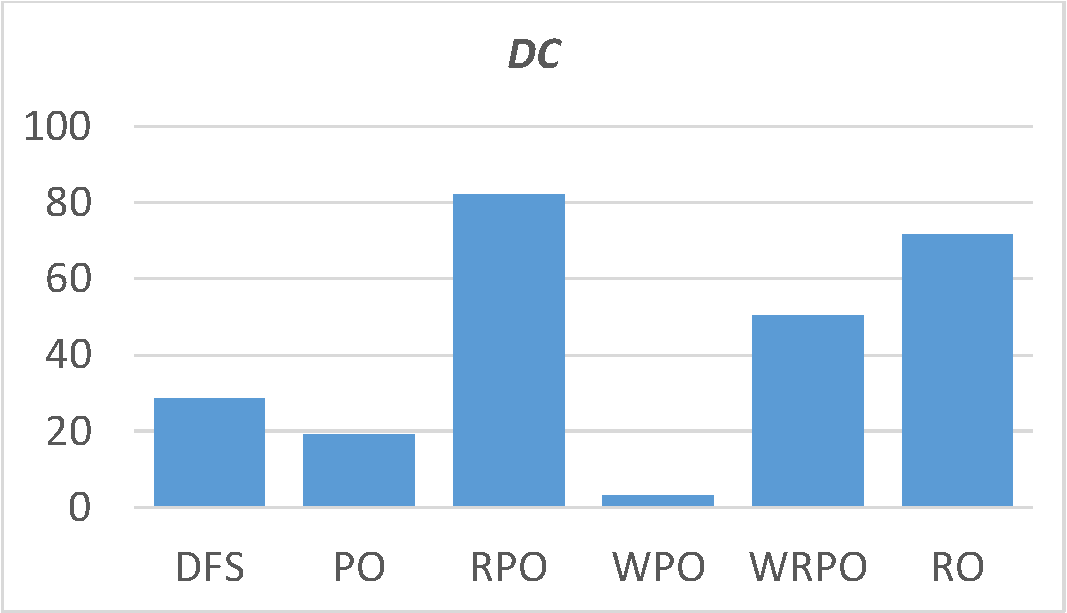
\includegraphics[width=0.32\linewidth]{ecoop-figures/dc-crop.pdf}
%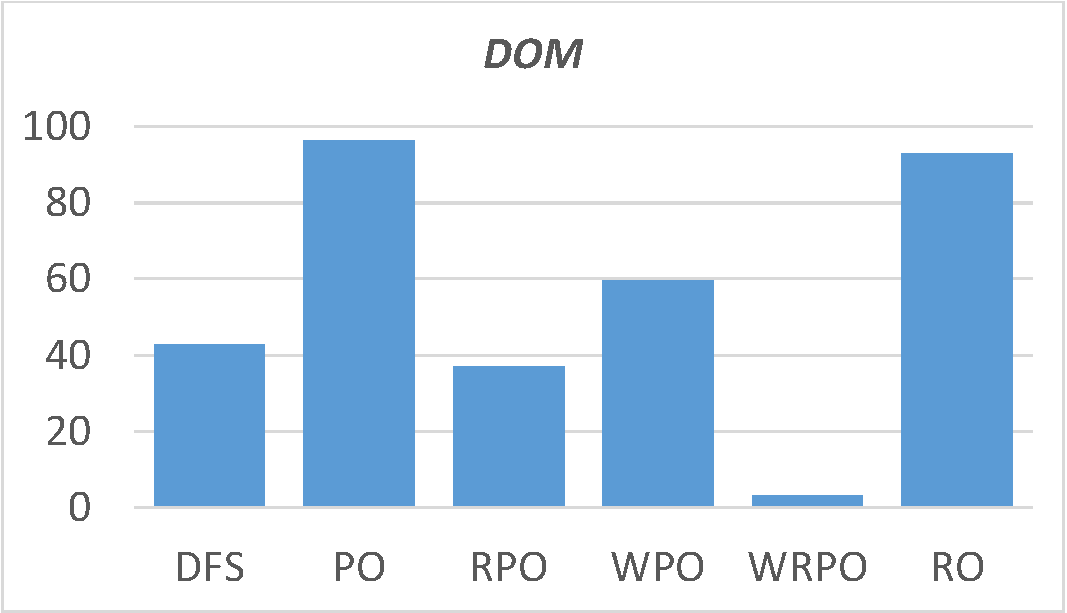
\includegraphics[width=0.32\linewidth]{ecoop-figures/dom-crop.pdf}
%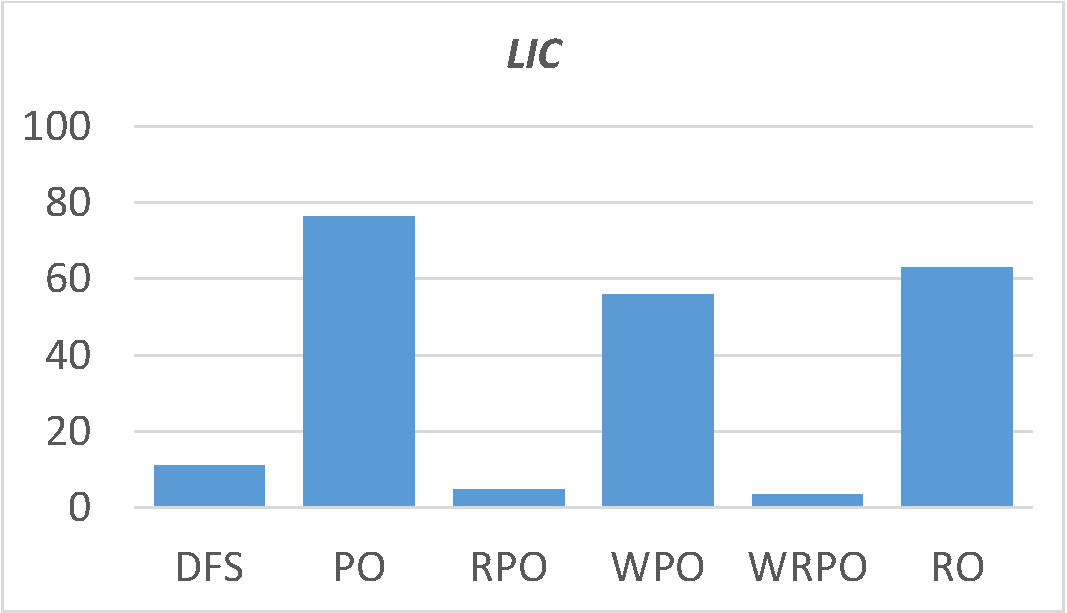
\includegraphics[width=0.32\linewidth]{ecoop-figures/lic-crop.pdf}
%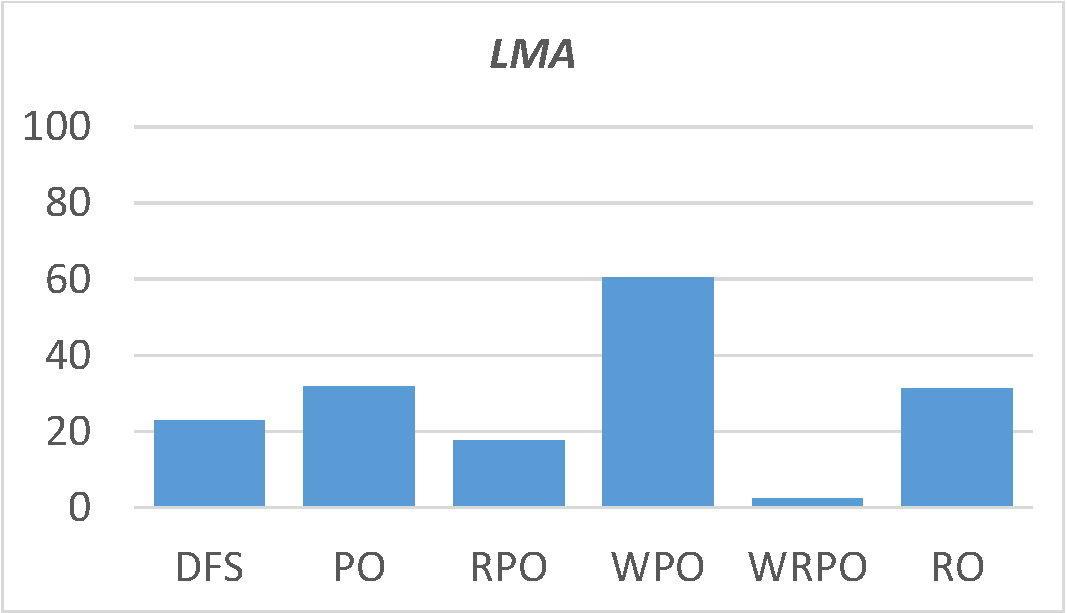
\includegraphics[width=0.32\linewidth]{ecoop-figures/lma-crop.pdf}
%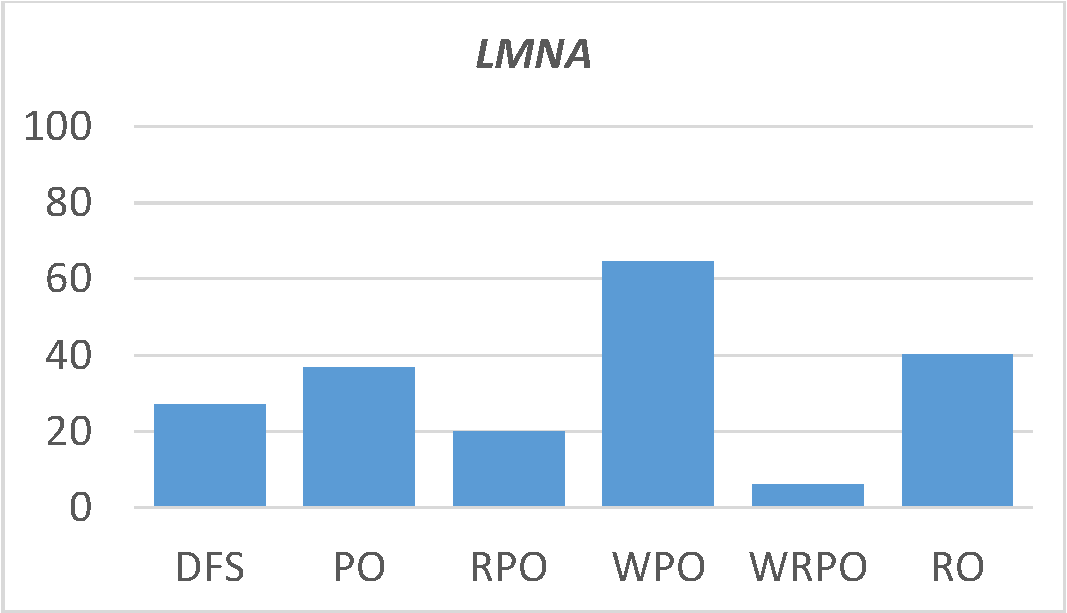
\includegraphics[width=0.32\linewidth]{ecoop-figures/lmna-crop.pdf}
%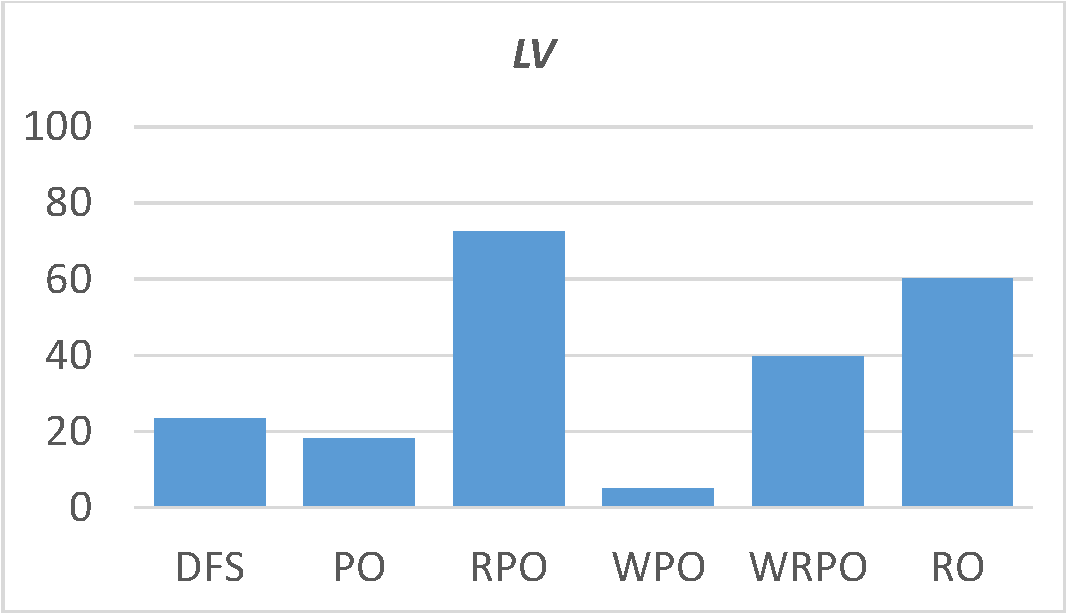
\includegraphics[width=0.32\linewidth]{ecoop-figures/lv-crop.pdf}
%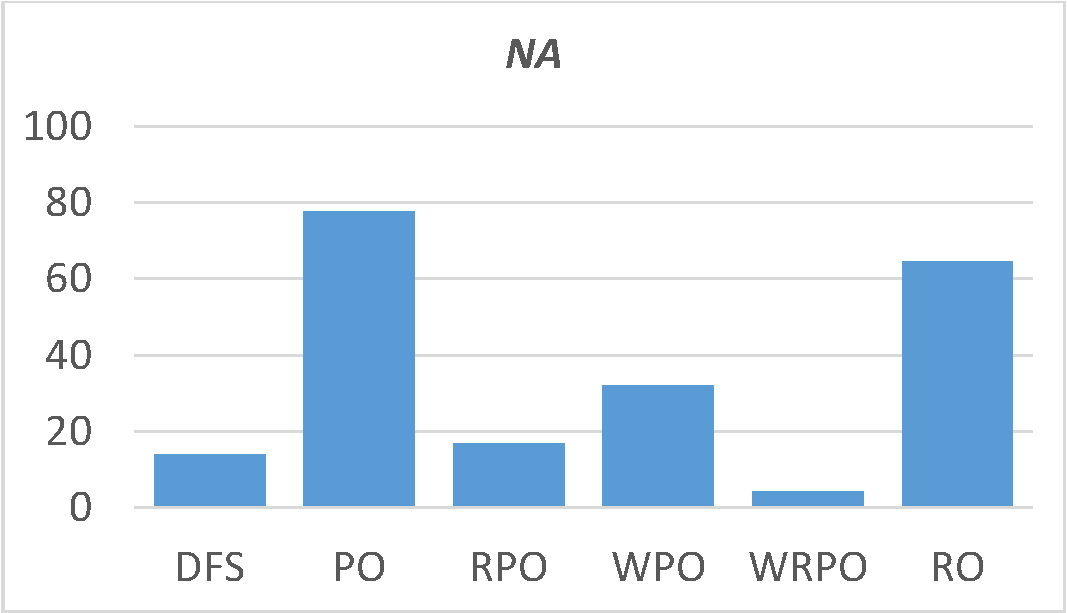
\includegraphics[width=0.32\linewidth]{ecoop-figures/na-crop.pdf}
%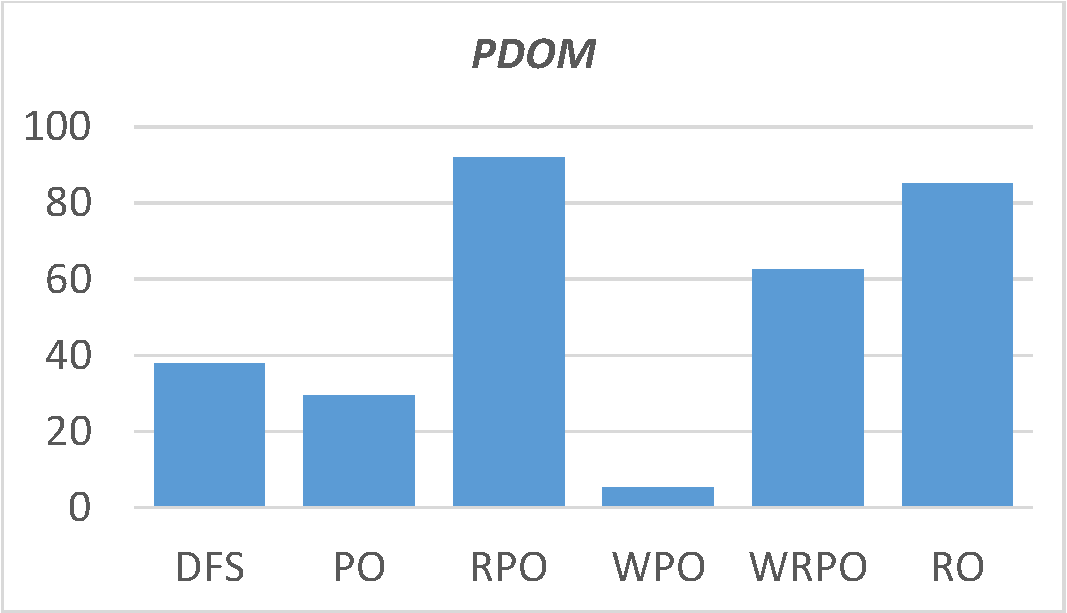
\includegraphics[width=0.32\linewidth]{ecoop-figures/pdom-crop.pdf}
%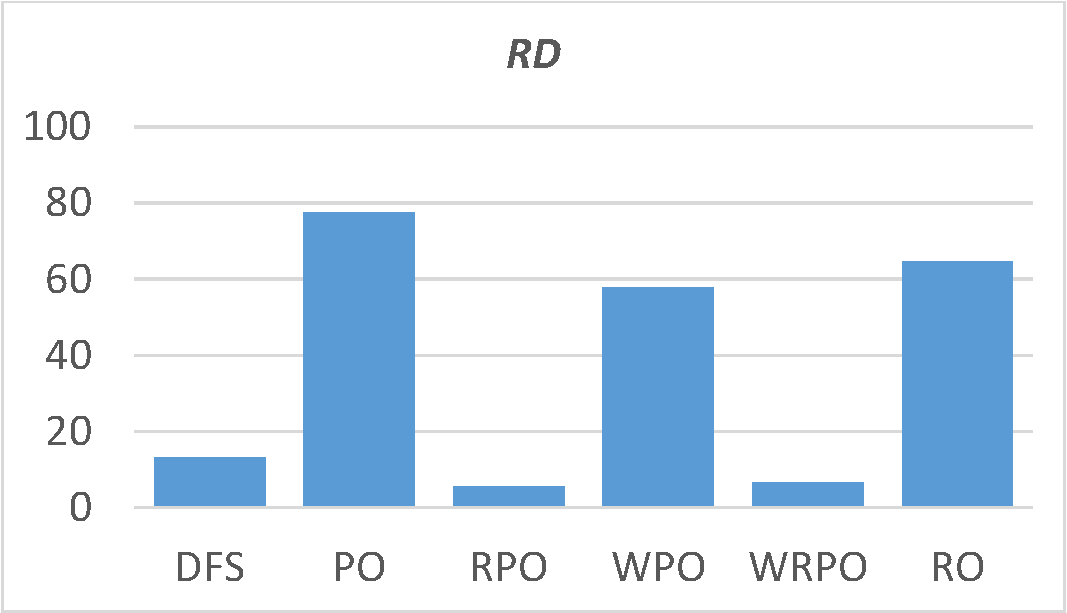
\includegraphics[width=0.32\linewidth]{ecoop-figures/rd-crop.pdf}
%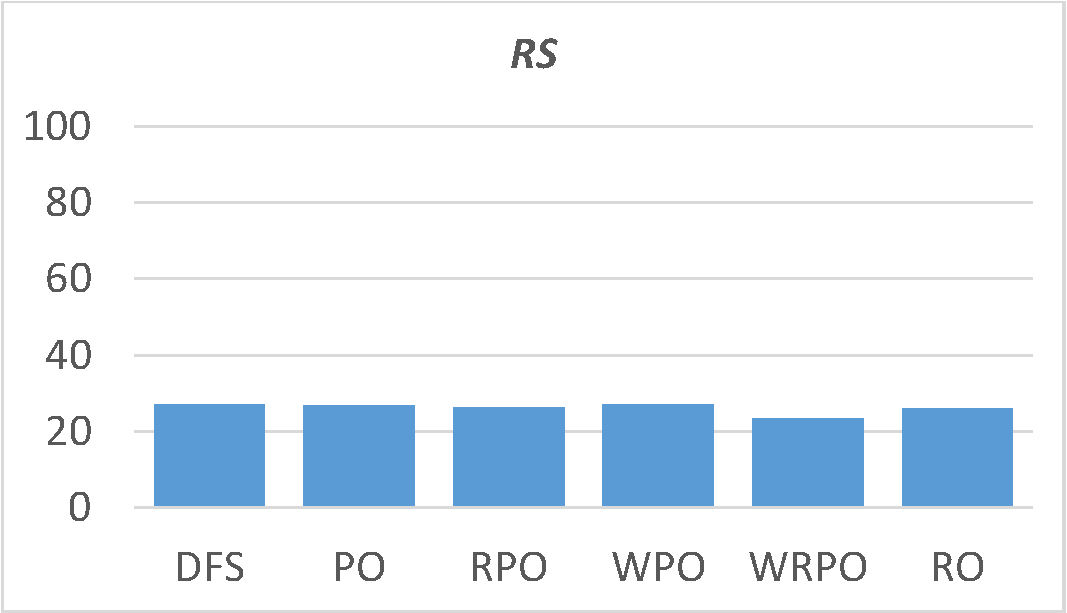
\includegraphics[width=0.32\linewidth]{ecoop-figures/rs-crop.pdf}
%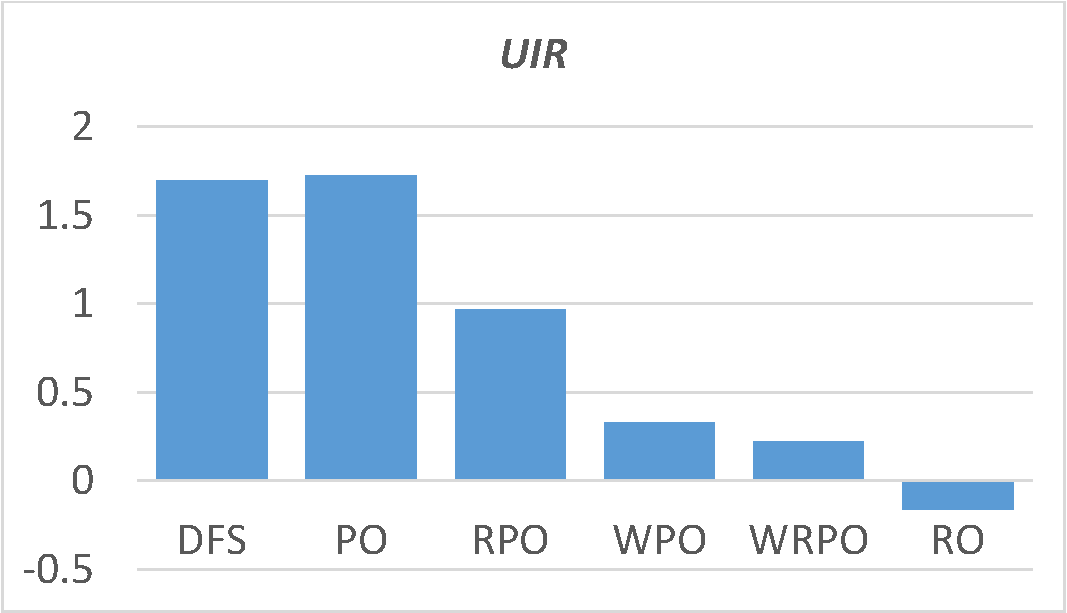
\includegraphics[width=0.32\linewidth]{ecoop-figures/uir-crop.pdf}
%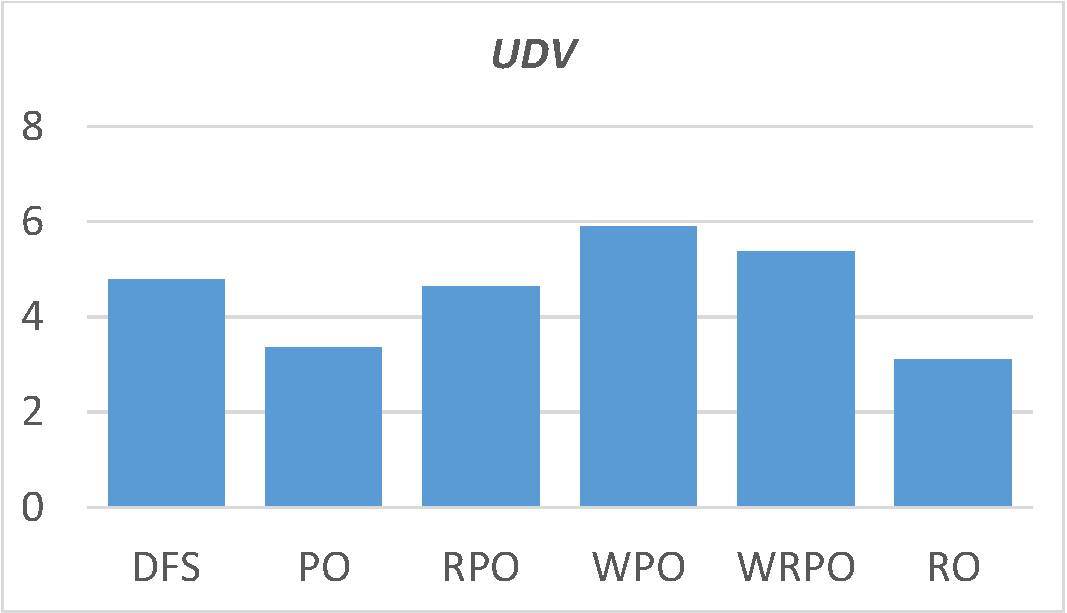
\includegraphics[width=0.32\linewidth]{ecoop-figures/udv-crop.pdf}
%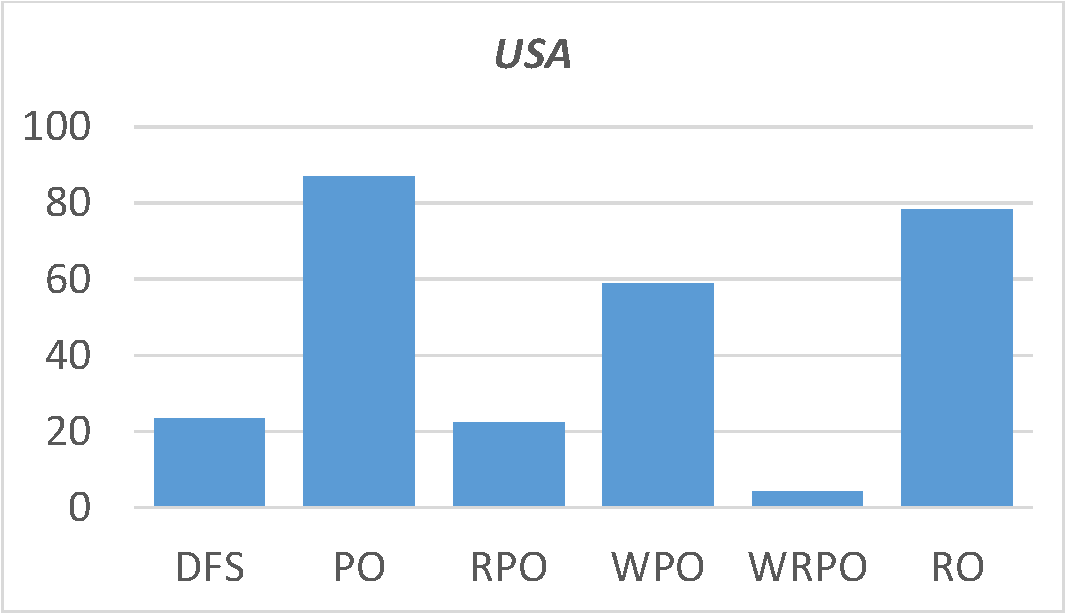
\includegraphics[width=0.32\linewidth]{ecoop-figures/usa-crop.pdf}
%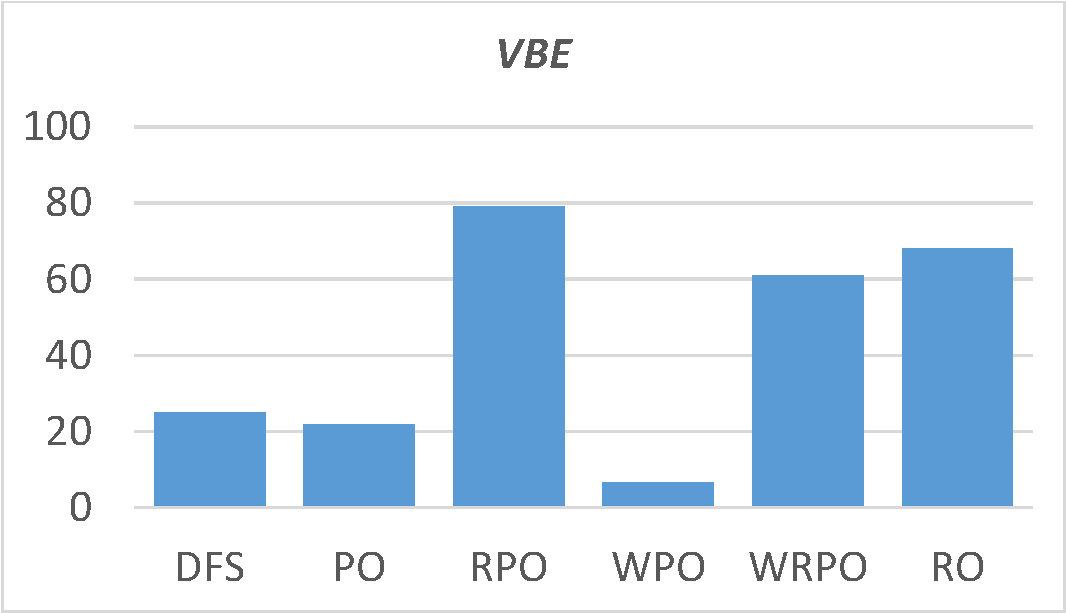
\includegraphics[width=0.32\linewidth]{ecoop-figures/vbe-crop.pdf}
%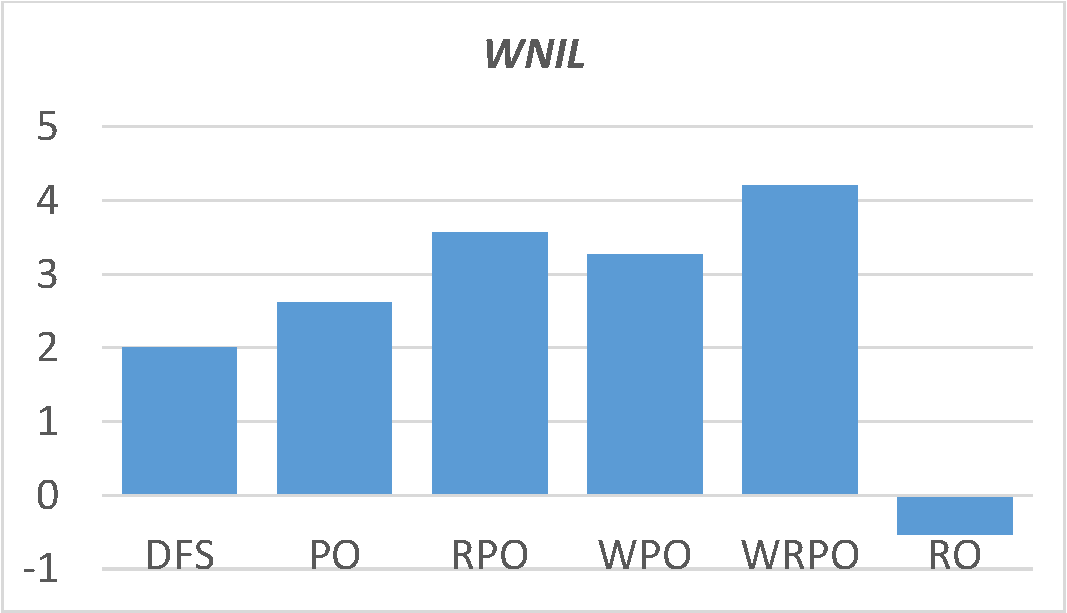
\includegraphics[width=0.32\linewidth]{ecoop-figures/wnil-crop.pdf}\newline
%\textbf{c) \textit{Overall}}\\
%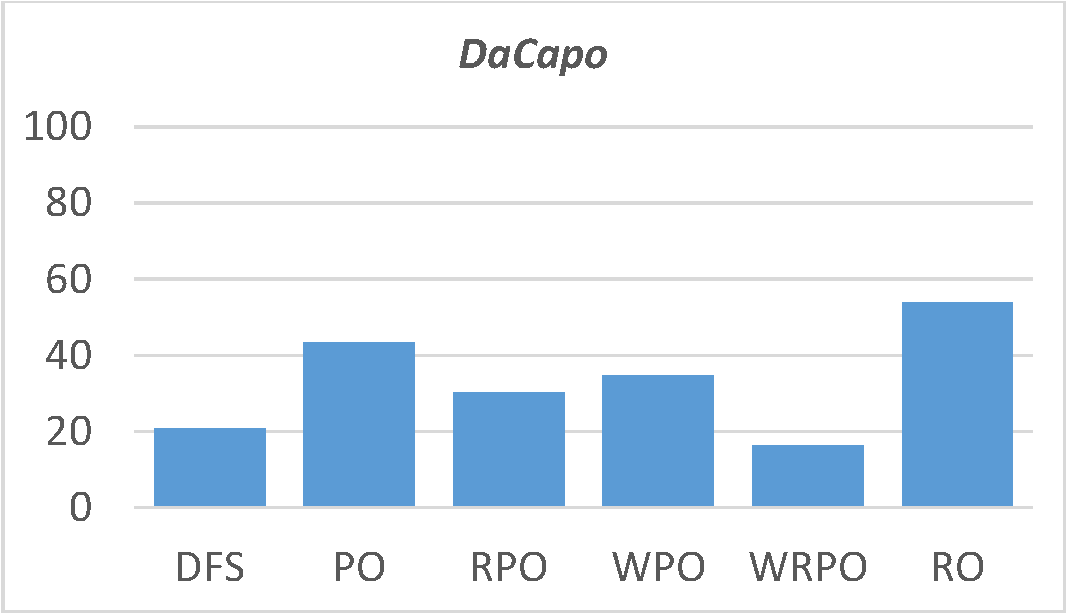
\includegraphics[width=0.32\linewidth]{ecoop-figures/dacapo-overall-crop.pdf}
  %\caption[Percentage reduction in execution time of hybrid approach over other candidate traversals on \textit{DaCapo} (Sequential mode) and \textit{SourceForge} (Cluster mode).]
%{Percentage reduction in execution time of hybrid approach over other candidate traversals on \textit{DaCapo} (Sequential mode) and \textit{SourceForge} (Cluster mode).
%\label{fig:dacapo-singlemachine-time-percentage}}
%\end{figure*}

%\begin{figure*}[ht!]
%\centering
%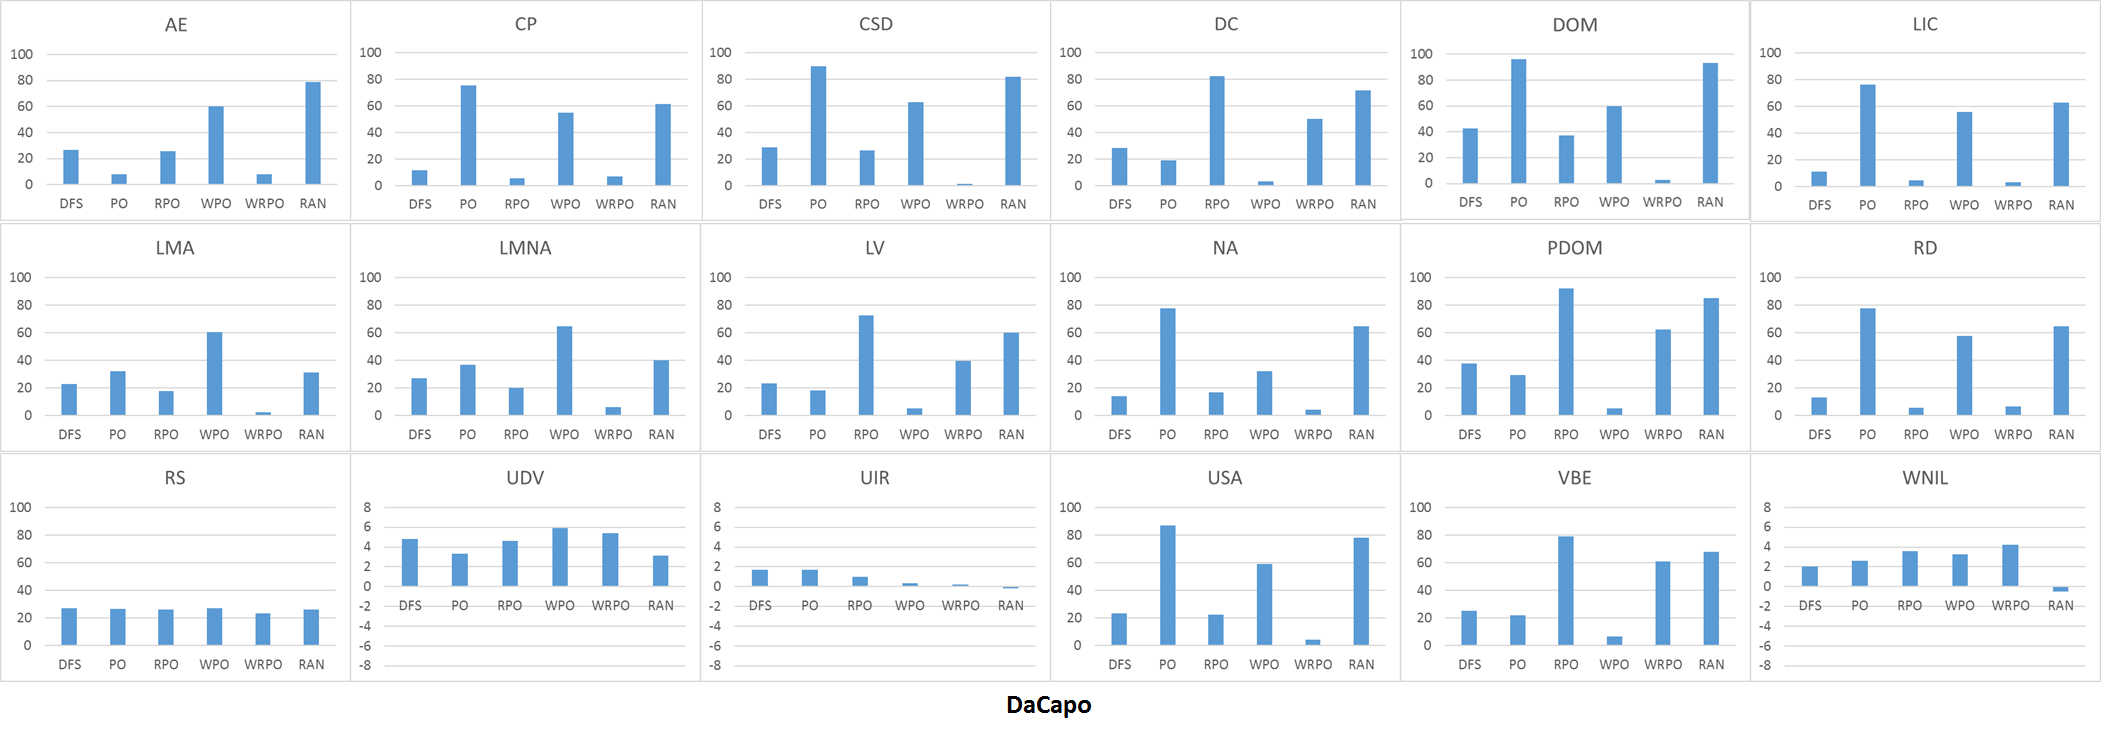
\includegraphics[width=\textwidth]{ecoop-figures/dacapo-seq-reduction.png}
%  \caption[Percentage reduction in execution time of hybrid approach over other candidate traversals on \textit{DaCapo} (Sequential mode), \textit{DaCapo} (Cluster mode), \textit{SourceForge} (Cluster mode).]
%{Percentage reduction in execution time of hybrid approach over other candidate traversals on \textit{DaCapo} (Sequential mode), \textit{DaCapo} (Cluster mode), \textit{SourceForge} (Cluster mode).
%\label{fig:dacapo-singlemachine-time-percentage}}
%\end{figure*}

\begin{figure}%
\centering
\scriptsize
\begin{tabular}{lrrrrrr|rrrrrr}
\toprule
\multicolumn{1}{l}{Analysis} & \multicolumn{1}{c|}{DaCapo}                    & \multicolumn{1}{c}{GitHub} \\
\midrule
\multicolumn{1}{l}{CP} & \cellcolor{lightblue}9\%  & \cellcolor{lightblue}5\%  \\
\multicolumn{1}{l}{CSD} & \cellcolor{lightblue}4\%  & \cellcolor{lightblack}12\% \\
\multicolumn{1}{l}{DC} & \cellcolor{lightblue}7\%  & \cellcolor{lightblue}7\%  \\
\multicolumn{1}{l}{LIC} & \cellcolor{lightblue}7\%  & \cellcolor{lightblack}19\% \\
\multicolumn{1}{l}{USA} & \cellcolor{lightblue}9\%  & \cellcolor{lightblue}9\% \\
\multicolumn{1}{l}{VFR} & \cellcolor{lightblack}15\%  & \cellcolor{lightblue}9\% \\
\multicolumn{1}{l}{MWN} & \cellcolor{lightblack}15\%  & \cellcolor{lightblue}9\% \\
\multicolumn{1}{l}{AE} & \cellcolor{lightblack}14\%  &  \cellcolor{lightblack}11\% \\
\multicolumn{1}{l}{DOM} & \cellcolor{lightblue}6\%  & \cellcolor{lightblue}6\% \\
\multicolumn{1}{l}{LMA} & \cellcolor{lightblue}6\%  & \cellcolor{lightblue}6\% \\
\multicolumn{1}{l}{LMNA} & \cellcolor{lightblue}9\%  & \cellcolor{lightblue}7\% \\
\multicolumn{1}{l}{LV} & \cellcolor{lightblack}11\%  & \cellcolor{lightblack}11\%  \\
\multicolumn{1}{l}{NA} & \cellcolor{lightblack}10\%  & \cellcolor{lightblack}10\%  \\
\multicolumn{1}{l}{PDOM} & \cellcolor{lightblack}10\%  & \cellcolor{lightblack}24\% \\
\multicolumn{1}{l}{RD} & \cellcolor{lightblue}9\%  & \cellcolor{lightblue}5\% \\
\multicolumn{1}{l}{RS} & \cellcolor{lightblack}28\%  & \cellcolor{lightblue}7\% \\
\multicolumn{1}{l}{VBE} & \cellcolor{lightblack}13\%  & \cellcolor{lightblack}10\% \\
\multicolumn{1}{l}{SS} & \cellcolor{lightblack}22\%  & \cellcolor{lightblack}10\%  \\
\multicolumn{1}{l}{UDV} &  \cellcolor{lightblue}3\%   &  \cellcolor{lightblue}0\%  \\
\multicolumn{1}{l}{UIR} &  \cellcolor{lightblue}0\%   &  \cellcolor{lightblue}0\%  \\
\multicolumn{1}{l}{WNIL} &  \cellcolor{lightblue}2\%   &  \cellcolor{lightblue}0\% \\
\bottomrule
\end{tabular}%
\caption{Reduction in running times against hand optimized analysis.}
\label{fig:reduction-oopsla}
\end{figure}
